\documentclass[tikz, border=6pt]{standalone}
\usepackage{tikz}
\usetikzlibrary{positioning}
\usepackage{physics}
\usepackage{siunitx}
\usepackage{ifthen}
\usepackage{tikz}
\usepackage[outline]{contour}
\usepackage{silence}

\usetikzlibrary{calc}
\usetikzlibrary{angles,quotes}
\usetikzlibrary{arrows.meta}
\usetikzlibrary{patterns}

\AtBeginDocument{\RenewCommandCopy\qty\SI}
\tikzset{>=latex}
\contourlength{1.4pt}

% -----------------------------------------------------------------------------
% Color palette
% -----------------------------------------------------------------------------
\colorlet{angleColor}{blue!70!black}
\colorlet{forceColor}{red!65!black}
\colorlet{forceComponentColor}{red!50!blue!80!black!80}
\colorlet{sensorTrackColor}{black!50}
\colorlet{signalOutputColor}{green!70!black}
\colorlet{supplyTerminalColor}{red!70!black}
\colorlet{groundTerminalColor}{blue!70!black}
% \colorlet{uColor}{green!50!black};
% \colorlet{omegaColor}{orange!90!black};
% \colorlet{tauColor}{green!80!black};

% -----------------------------------------------------------------------------
% Reusable drawing styles (used by pendulum.tex)
% -----------------------------------------------------------------------------
\tikzset{
  supportSurface/.style={
    preaction={fill,top color=black!10,bottom color=black!5,shading angle=20},
    fill,
    pattern=north east lines,
    draw=none,
    minimum width=0.3,
    minimum height=0.6
  },
  forceVector/.style={
    ->,
    forceColor,
    very thick,
    line cap=round
  },
  information text/.style={
    rounded corners,
    fill=red!10,
    inner sep=1ex
  }
}


\begin{document}
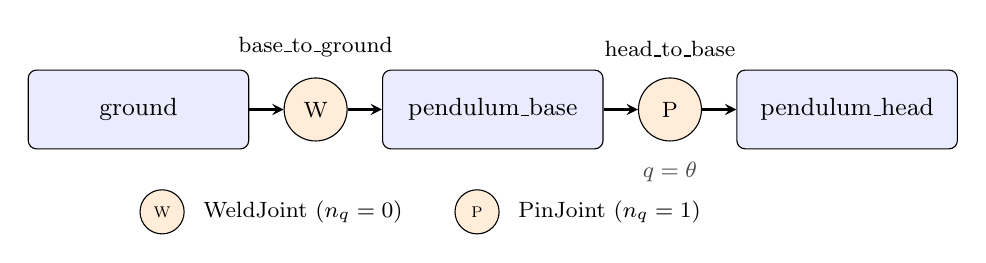
\begin{tikzpicture}[
    body/.style={
        draw, rounded corners=3pt, minimum width=28mm, minimum height=10mm,
        fill=blue!8, font=\small
    },
    joint/.style={
        draw, circle, minimum size=8mm, fill=orange!15, font=\footnotesize,
        inner sep=1pt
    },
    conn/.style={->, thick, >=stealth},
    coord/.style={font=\footnotesize\itshape, text=black!70},
]

% Bodies
\node[body] (ground)  at (0,0)    {ground};
\node[body] (base)    at (4.5,0)  {pendulum\_base};
\node[body] (head)    at (9,0)    {pendulum\_head};

% Joints
\node[joint] (weld) at (2.25,0) {W};
\node[joint] (pin)  at (6.75,0) {P};

% Connections
\draw[conn] (ground.east) -- (weld);
\draw[conn] (weld)        -- (base.west);
\draw[conn] (base.east)   -- (pin);
\draw[conn] (pin)          -- (head.west);

% Joint labels
\node[above=4pt of weld, font=\footnotesize] {base\_to\_ground};
\node[above=4pt of pin,  font=\footnotesize] {head\_to\_base};

% Generalized coordinate
\node[coord, below=4pt of pin] {$q = \theta$};

% Legend
\node[joint, scale=0.7] at (0.3,-1.3) {W};
\node[font=\footnotesize, anchor=west] at (0.7,-1.3) {WeldJoint ($n_q = 0$)};
\node[joint, scale=0.7] at (4.3,-1.3) {P};
\node[font=\footnotesize, anchor=west] at (4.7,-1.3) {PinJoint ($n_q = 1$)};

\end{tikzpicture}
\end{document}

